\documentclass[10pt]{beamer}\usepackage[]{graphicx}\usepackage[]{color}
%% maxwidth is the original width if it is less than linewidth
%% otherwise use linewidth (to make sure the graphics do not exceed the margin)
\makeatletter
\def\maxwidth{ %
  \ifdim\Gin@nat@width>\linewidth
    \linewidth
  \else
    \Gin@nat@width
  \fi
}
\makeatother

\definecolor{fgcolor}{rgb}{0.345, 0.345, 0.345}
\newcommand{\hlnum}[1]{\textcolor[rgb]{0.686,0.059,0.569}{#1}}%
\newcommand{\hlstr}[1]{\textcolor[rgb]{0.192,0.494,0.8}{#1}}%
\newcommand{\hlcom}[1]{\textcolor[rgb]{0.678,0.584,0.686}{\textit{#1}}}%
\newcommand{\hlopt}[1]{\textcolor[rgb]{0,0,0}{#1}}%
\newcommand{\hlstd}[1]{\textcolor[rgb]{0.345,0.345,0.345}{#1}}%
\newcommand{\hlkwa}[1]{\textcolor[rgb]{0.161,0.373,0.58}{\textbf{#1}}}%
\newcommand{\hlkwb}[1]{\textcolor[rgb]{0.69,0.353,0.396}{#1}}%
\newcommand{\hlkwc}[1]{\textcolor[rgb]{0.333,0.667,0.333}{#1}}%
\newcommand{\hlkwd}[1]{\textcolor[rgb]{0.737,0.353,0.396}{\textbf{#1}}}%
\let\hlipl\hlkwb

\usepackage{framed}
\makeatletter
\newenvironment{kframe}{%
 \def\at@end@of@kframe{}%
 \ifinner\ifhmode%
  \def\at@end@of@kframe{\end{minipage}}%
  \begin{minipage}{\columnwidth}%
 \fi\fi%
 \def\FrameCommand##1{\hskip\@totalleftmargin \hskip-\fboxsep
 \colorbox{shadecolor}{##1}\hskip-\fboxsep
     % There is no \\@totalrightmargin, so:
     \hskip-\linewidth \hskip-\@totalleftmargin \hskip\columnwidth}%
 \MakeFramed {\advance\hsize-\width
   \@totalleftmargin\z@ \linewidth\hsize
   \@setminipage}}%
 {\par\unskip\endMakeFramed%
 \at@end@of@kframe}
\makeatother

\definecolor{shadecolor}{rgb}{.97, .97, .97}
\definecolor{messagecolor}{rgb}{0, 0, 0}
\definecolor{warningcolor}{rgb}{1, 0, 1}
\definecolor{errorcolor}{rgb}{1, 0, 0}
\newenvironment{knitrout}{}{} % an empty environment to be redefined in TeX

\usepackage{alltt}

\usepackage{graphicx, color}
\usepackage{alltt}
\usepackage{booktabs, calc, rotating}
\usepackage[round]{natbib}
\usepackage{pdfpages, subfigure}
\usepackage{multicol}
\usepackage{amsmath, amsbsy, amssymb, amsthm, graphicx}
\usepackage[english]{babel}
\usepackage{xkeyval} 
\usepackage{xfrac}
\usepackage{multicol}
\usepackage[normalem]{ulem}
\usepackage{multirow, fancyvrb} 
\usepackage{tikz, geometry, tkz-graph, xcolor}
\usepackage{listings}

\let\oldemptyset\emptyset
\let\emptyset\varnothing

\renewenvironment{knitrout}{\setlength{\topsep}{-.2mm}}{}

\usetikzlibrary{arrows,positioning} 
\tikzset{
  % Define standard arrow tip
  >=stealth',
  % Define style for boxes
  punkt/.style={
    rectangle,
    rounded corners,
    draw=black, very thick,
    text width=6.5em,
    minimum height=2em,
    text centered},
  % Define arrow style
  pil/.style={
    ->,
    thick,
    shorten <=2pt,
    shorten >=2pt,}
}
\usetikzlibrary{trees}
% Set the overall layout of the tree
\tikzstyle{level 1}=[level distance=2.5cm, sibling distance=4cm] 
\tikzstyle{level 2}=[level distance=2.5cm, sibling distance=2.5cm]
\tikzstyle{level 3}=[level distance=2.5cm, sibling distance=1cm]

% Define styles for bags and leafs
\tikzstyle{bag} = [text width=4em, text centered]
\tikzstyle{end} = [circle, minimum width=3pt,fill, inner sep=0pt]
\tikzstyle{openend} = [circle, minimum width=3pt, inner sep=0pt]

\hypersetup{colorlinks, citecolor=blue, linkcolor=., menucolor=white, filecolor=blue, anchorcolor=yellow}

\usetikzlibrary{arrows,positioning} 
\tikzset{
  % Define standard arrow tip
  >=stealth',
  % Define style for boxes
  punkt/.style={rectangle, rounded corners, draw=black, very thick, text width=6.5em, 
    minimum height=2em, text centered},
  % Define arrow style
  pil/.style={ ->, thick, shorten <=2pt, shorten >=2pt,}}

\graphicspath{{figure/}}

\newcommand{\cov}{\mathrm{cov}}
\newcommand{\dif}{\mathrm{d}}
\newcommand{\bigbrk}{\vspace*{2in}}
\newcommand{\smallbrk}{\vspace*{.1in}}
\newcommand{\midbrk}{\vspace*{1in}}
\newcommand{\red}[1]{{\color{red}#1}}
\newcommand{\empr}[1]{{\emph{\color{red}#1}}}
\newcommand{\blue}[1]{{\color{blue}#1}}
\newcommand{\green}[1]{{\color{green}#1}}
\newcommand{\pkg}[1]{{\textbf{\texttt{#1}}}}
\newcommand{\code}[1]{{\texttt{#1}}}
\newcommand{\calc}[1]{{\fbox{\mbox{#1}}}}
\newcommand{\Var}{\mathrm{Var}}%
\newcommand{\var}{\mathrm{var}}%
\newcommand{\V}{\mathrm{V}}%
\newcommand{\R}{\texttt{R} }%
\newcommand{\Cov}{\mathrm{Cov}}%

\mode<presentation> {
  \usetheme{UTD}
  \usecolortheme[RGB={200,0,0}]{structure}
  \setbeamercovered{transparent}
}

\usepackage[latin1]{inputenc}
\usepackage{times}
\usepackage[T1]{fontenc}

\DeclareSymbolFont{extraup}{U}{zavm}{m}{n}
\DeclareMathSymbol{\varheart}{\mathalpha}{extraup}{86}
\DeclareMathSymbol{\vardiamond}{\mathalpha}{extraup}{87}

\newcommand*{\mybox}[1]{\framebox{#1}}

\title[STAT 6390]{STAT 6390: Analysis of Survival Data\\
  \small{Textbook coverage: Chapter 1}\\}
\author[Steven Chiou]{Steven Chiou}
\institute[UTD]{Department of Mathematical Sciences, \\ University of Texas at Dallas}
\date{}

% UTD logo on top right corner
% \usepackage[absolute, overlay]{textpos}
% \addtobeamertemplate{frametitle}{}{%
% \begin{textblock*}{100cm}(.94\textwidth, 0.6cm)
%   \includegraphics[trim = 1.8cm .9cm 1.8cm .92cm, clip, scale = .28, keepaspectratio]{UTDlogo}
% \end{textblock*}}
\IfFileExists{upquote.sty}{\usepackage{upquote}}{}
\begin{document}

\begin{frame}[fragile]
  \titlepage

\end{frame}

\setbeamercolor*{item}{fg=red}
\bgroup
\usebackgroundtemplate{%
  \tikz[overlay,remember picture] \node[opacity=0.05, at=(current page.center)] {
    
\includegraphics[height=\paperheight,width=\paperwidth]{UTDbg}};}

\section{Introduction}
\begin{frame}
  \frametitle{Survival analysis?}
  \begin{itemize}
  \item Survival analysis aka
    \begin{itemize}
    \item duration analysis
    \item event history analysis
    \item time to event analysis
    \end{itemize}
  \item Models the relationship between duration ($Y$) and covariates ($X$).
    \begin{itemize}
    \item time until graduation
    \item time until failure of  an electronic component
    \item time until a patient dies
    \end{itemize}
  \item Linear regression, e.g., ordinary least squares \texttt{lm(Y $\sim$ X)}, is usually not feasible.
  \end{itemize}
\end{frame}

\begin{frame}
  \frametitle{Why not use OLS?}
  \begin{itemize}
  \item Inference for OLS assumes $Y$ is normal.
    \begin{itemize}
    \item Duration is always positive.
    \item Duration is usually not-normal.
    \item Log-transformation might not work.
    \end{itemize}
    \centering
    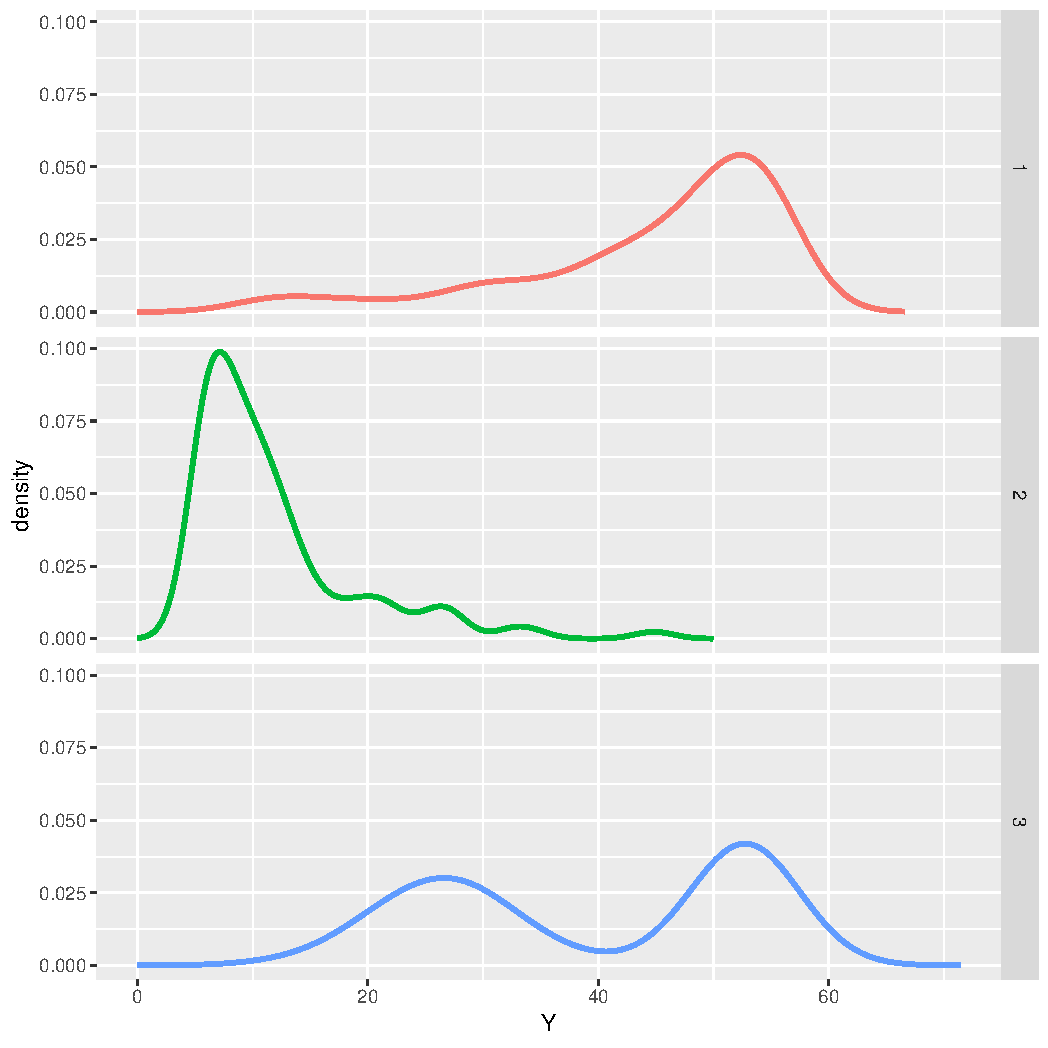
\includegraphics[scale = .28]{note1-1}\hspace{.5cm}
    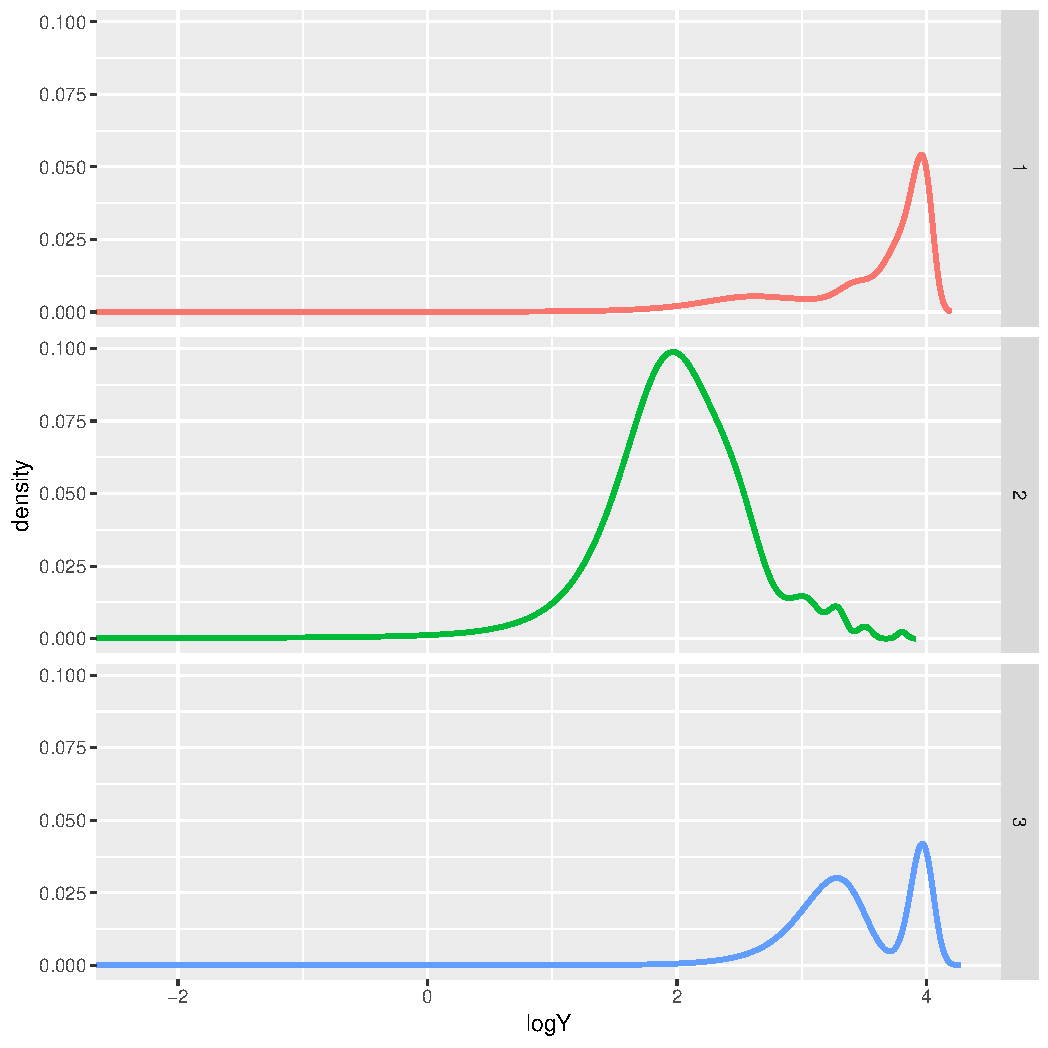
\includegraphics[scale = .28]{note1-2}
  \end{itemize}
\end{frame}


\begin{frame}
  \frametitle{Why not use OLS?}
  \begin{itemize}
  \item OLS handles missing values via complete case analysis or imputation*.
    \begin{itemize}
    \item Survival data consists of missing values that are meaningful, 
      so dropping incomplete observations means losing information. 
    \item Imputation requires additional assumption from the distribution of $Y$.
    \item Replacing missing values with mean or median would result in 
      underestimation if the missingness are caused by \emph{right censoring}.
    \end{itemize}
  \item Common source of missing values in survival data: \emph{censoring} and \emph{truncation}.
  \end{itemize}
\end{frame}

\begin{frame}
  \frametitle{Other reasons for survival models}
  \begin{itemize}
  \item Survival models can handle time-varying covaraites.
  \item Probabilities associated with survival times is more relevant.
  \item Many existing packages make routine survival analysis more accessible.
  \item A partial list of \R package can be found here:
    \url{https://cran.r-project.org/web/views/Survival.html}
  \end{itemize}
\end{frame}

\section{Censoring}

\begin{frame}
  \frametitle{Censoring}
  \begin{itemize}
  % \item \empr{Right censor} is the most common type of censoring in survival analysis. 
  \item The survival time of an individual is said to be \empr{right censored} when the end-point 
    of interest has not been observed for that individual. 
  \item The ``end-point'' is a well-defined event, say death from a disease.
  \item The actually survival time can be regarded as right censored when
    \begin{itemize}
    \item lost to follow-up
    \item death from a different cause
      \item no event had occurred by the end of the study 
    \end{itemize}
  \end{itemize}
\end{frame}
  

\begin{frame}[fragile]
  \frametitle{Loading \texttt{survMisc}, Ver 0.4.6.}
  \begin{itemize}
  %% \item We will see this through the Worcester Heart Attach Study (WHAS).
  \item Most datasets in the book are available via \R package \pkg{survMisc}, 
    version 0.4.6 or eariler. 
  \item Archived \R package can be installed as follows
\begin{knitrout}\scriptsize
\definecolor{shadecolor}{rgb}{0.969, 0.969, 0.969}\color{fgcolor}\begin{kframe}
\begin{alltt}
\hlstd{> }\hlcom{## install.package("devtools")}
\hlstd{> }\hlkwd{library}\hlstd{(devtools)}
\hlstd{> }\hlkwd{install_version}\hlstd{(}\hlstr{"survMisc"}\hlstd{,} \hlkwc{version} \hlstd{=} \hlstr{"0.4.6"}\hlstd{)}
\end{alltt}
\end{kframe}
\end{knitrout}
  \item \texttt{install.package()} installs the latest version.
  \item \texttt{install\_version()} installs a specified package.
  \end{itemize}
\end{frame}

\begin{frame}[fragile]
  \frametitle{WHAS}
  \begin{itemize}
  \item Load data from Worcester Heart Attach Study (WHAS) in Table 1.1:
\begin{knitrout}\scriptsize
\definecolor{shadecolor}{rgb}{0.969, 0.969, 0.969}\color{fgcolor}\begin{kframe}
\begin{alltt}
\hlstd{> }\hlkwd{data}\hlstd{(whas100,} \hlkwc{package} \hlstd{=} \hlstr{"survMisc"}\hlstd{)}
\end{alltt}
\end{kframe}
\end{knitrout}
  \item The above code only works with \pkg{survMisc} version $\le$0.4.6.

\begin{knitrout}\scriptsize
\definecolor{shadecolor}{rgb}{0.969, 0.969, 0.969}\color{fgcolor}\begin{kframe}
\begin{alltt}
\hlstd{> }\hlkwd{head}\hlstd{(whas100)}
\end{alltt}
\begin{verbatim}
  id admitdate   foldate los lenfol fstat age gender      bmi
1  1 3/13/1995 3/19/1995   4      6     1  65      0 31.38134
2  2 1/14/1995 1/23/1996   5    374     1  88      1 22.65790
3  3 2/17/1995 10/4/2001   5   2421     1  77      0 27.87892
4  4  4/7/1995 7/14/1995   9     98     1  81      1 21.47878
5  5  2/9/1995 5/29/1998   4   1205     1  78      0 30.70601
6  6 1/16/1995 9/11/2000   7   2065     1  82      1 26.45294
\end{verbatim}
\end{kframe}
\end{knitrout}
%% \item \texttt{admitdate} is the admission date.
%% \item \texttt{foldate} is the follow-up (last contact) date.
%% \item \texttt{fstat} is the follow-up status (1 = dead; 0 = alive).
\item A description of \texttt{whas100} can be called from
\begin{knitrout}\scriptsize
\definecolor{shadecolor}{rgb}{0.969, 0.969, 0.969}\color{fgcolor}\begin{kframe}
\begin{alltt}
\hlstd{> }\hlopt{?}\hlstd{whas100}
\hlstd{> }\hlopt{?}\hlstd{survMisc}\hlopt{::}\hlstd{whas100}
\end{alltt}
\end{kframe}
\end{knitrout}
   \item \texttt{whas100} is a \texttt{data.frame}. 
\begin{knitrout}\scriptsize
\definecolor{shadecolor}{rgb}{0.969, 0.969, 0.969}\color{fgcolor}\begin{kframe}
\begin{alltt}
\hlstd{> }\hlkwd{class}\hlstd{(whas100)}
\end{alltt}
\begin{verbatim}
[1] "data.frame"
\end{verbatim}
\end{kframe}
\end{knitrout}
  \end{itemize}
\end{frame}

\begin{frame}[fragile]
\frametitle{WHAS}
  \begin{itemize}
  \item A more effective way to manipulate data frame is through ``\texttt{tibble}''.
  \item Install \pkg{tidyverse} (\url{https://www.tidyverse.org})
\begin{knitrout}\scriptsize
\definecolor{shadecolor}{rgb}{0.969, 0.969, 0.969}\color{fgcolor}\begin{kframe}
\begin{alltt}
\hlstd{> }\hlcom{## install.package(tidyverse)}
\hlstd{> }\hlkwd{library}\hlstd{(tidyverse)}
\hlstd{> }\hlstd{whas100} \hlkwb{<-} \hlkwd{as.tibble}\hlstd{(whas100)}
\hlstd{> }\hlstd{whas100}
\end{alltt}
\begin{verbatim}
# A tibble: 100 x 9
      id admitdate  foldate      los lenfol fstat   age gender   bmi
   <int> <fct>      <fct>      <int>  <int> <int> <int>  <int> <dbl>
 1     1 3/13/1995  3/19/1995      4      6     1    65      0  31.4
 2     2 1/14/1995  1/23/1996      5    374     1    88      1  22.7
 3     3 2/17/1995  10/4/2001      5   2421     1    77      0  27.9
 4     4 4/7/1995   7/14/1995      9     98     1    81      1  21.5
 5     5 2/9/1995   5/29/1998      4   1205     1    78      0  30.7
 6     6 1/16/1995  9/11/2000      7   2065     1    82      1  26.5
 7     7 1/17/1995  10/15/1997     3   1002     1    66      1  35.7
 8     8 11/15/1994 11/24/2000    56   2201     1    81      1  28.3
 9     9 8/18/1995  2/23/1996      5    189     1    76      0  27.1
10    10 7/22/1995  12/31/2002     9   2719     0    40      0  21.8
# ... with 90 more rows
\end{verbatim}
\end{kframe}
\end{knitrout}
  \end{itemize}
\end{frame}

\begin{frame}[fragile]
\frametitle{WHAS}
  \begin{itemize}
  \item A transposed version to print \texttt{whas100}:
\begin{knitrout}\scriptsize
\definecolor{shadecolor}{rgb}{0.969, 0.969, 0.969}\color{fgcolor}\begin{kframe}
\begin{alltt}
\hlstd{> }\hlcom{## install.package(tidyverse)}
\hlstd{> }\hlkwd{glimpse}\hlstd{(whas100)}
\end{alltt}
\begin{verbatim}
Observations: 100
Variables: 9
$ id        <int> 1, 2, 3, 4, 5, 6, 7, 8, 9, 10, 11, 12, 13, 14, 15, 1...
$ admitdate <fct> 3/13/1995, 1/14/1995, 2/17/1995, 4/7/1995, 2/9/1995,...
$ foldate   <fct> 3/19/1995, 1/23/1996, 10/4/2001, 7/14/1995, 5/29/199...
$ los       <int> 4, 5, 5, 9, 4, 7, 3, 56, 5, 9, 6, 11, 6, 10, 7, 5, 6...
$ lenfol    <int> 6, 374, 2421, 98, 1205, 2065, 1002, 2201, 189, 2719,...
$ fstat     <int> 1, 1, 1, 1, 1, 1, 1, 1, 1, 0, 0, 1, 1, 0, 0, 0, 1, 1...
$ age       <int> 65, 88, 77, 81, 78, 82, 66, 81, 76, 40, 73, 83, 64, ...
$ gender    <int> 0, 1, 0, 1, 0, 1, 1, 1, 0, 0, 1, 0, 1, 0, 0, 0, 0, 0...
$ bmi       <dbl> 31.38134, 22.65790, 27.87892, 21.47878, 30.70601, 26...
\end{verbatim}
\end{kframe}
\end{knitrout}
  \item See \url{https://r4ds.had.co.nz/tibbles.html} for details.
  \end{itemize}
\end{frame}

\begin{frame}[fragile]
\frametitle{WHAS}
  \begin{itemize}
  \item Here is the screen shot of Table 1.1:
    \begin{center}
      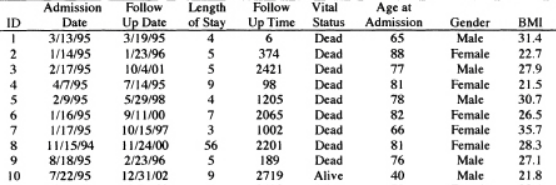
\includegraphics[trim = 0 0 0 .1cm, clip, scale = .45]{tab1-1}
    \end{center}
  \item \texttt{los} corresponds to length of stay
  \item \texttt{fstat} corresponds to the vital status; this is also called the \empr{status indicator}, 
    or the \empr{censoring indicator}.
    \begin{itemize}
    \item It talks the value of 1 if an event has observed (death) and 0 otherwise.
    \end{itemize}
  \end{itemize}
\end{frame}

\begin{frame}[fragile]
\frametitle{WHAS}
  \begin{itemize}
  \item There are common two ways to display follow-up times
  \end{itemize}
  \begin{center}
    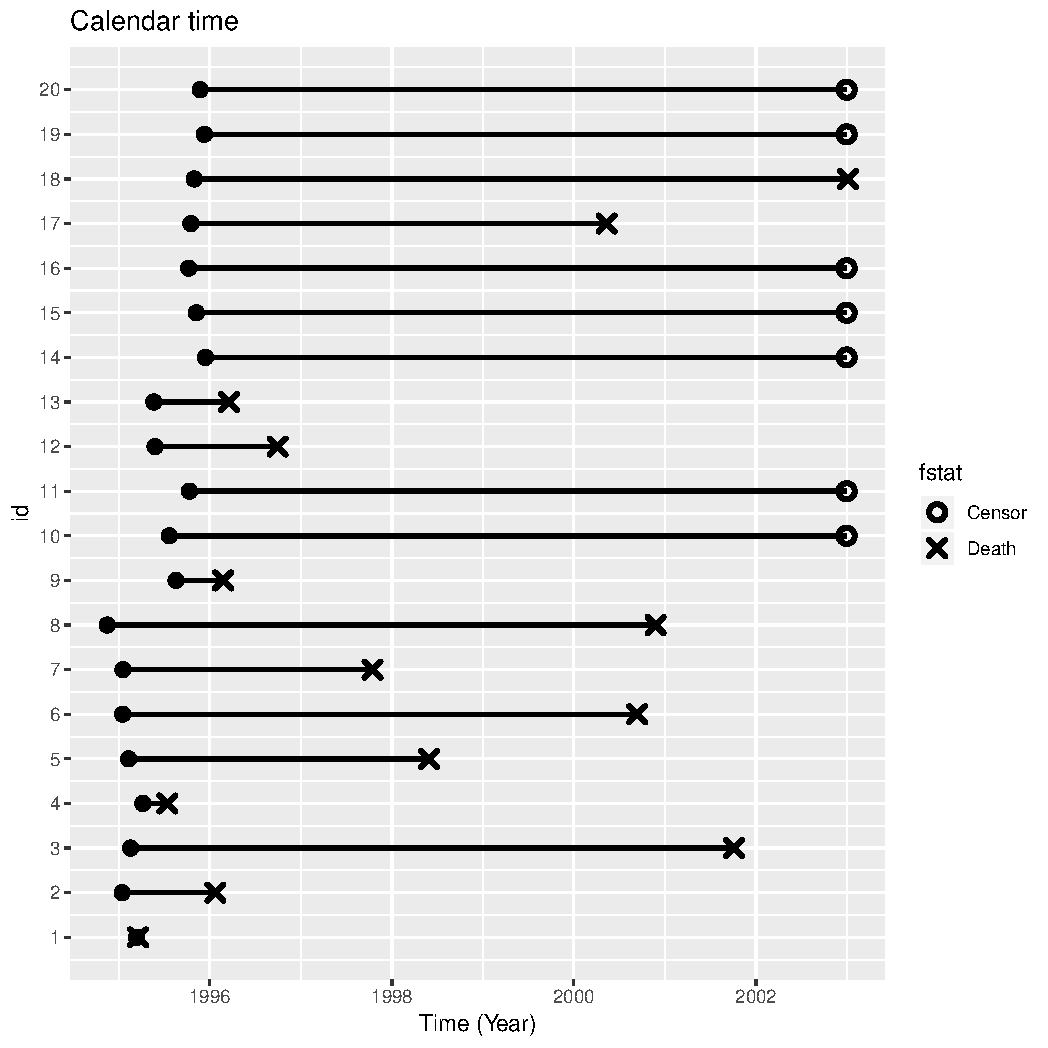
\includegraphics[scale = .3]{tab1-1-1}\hspace{.5cm}
    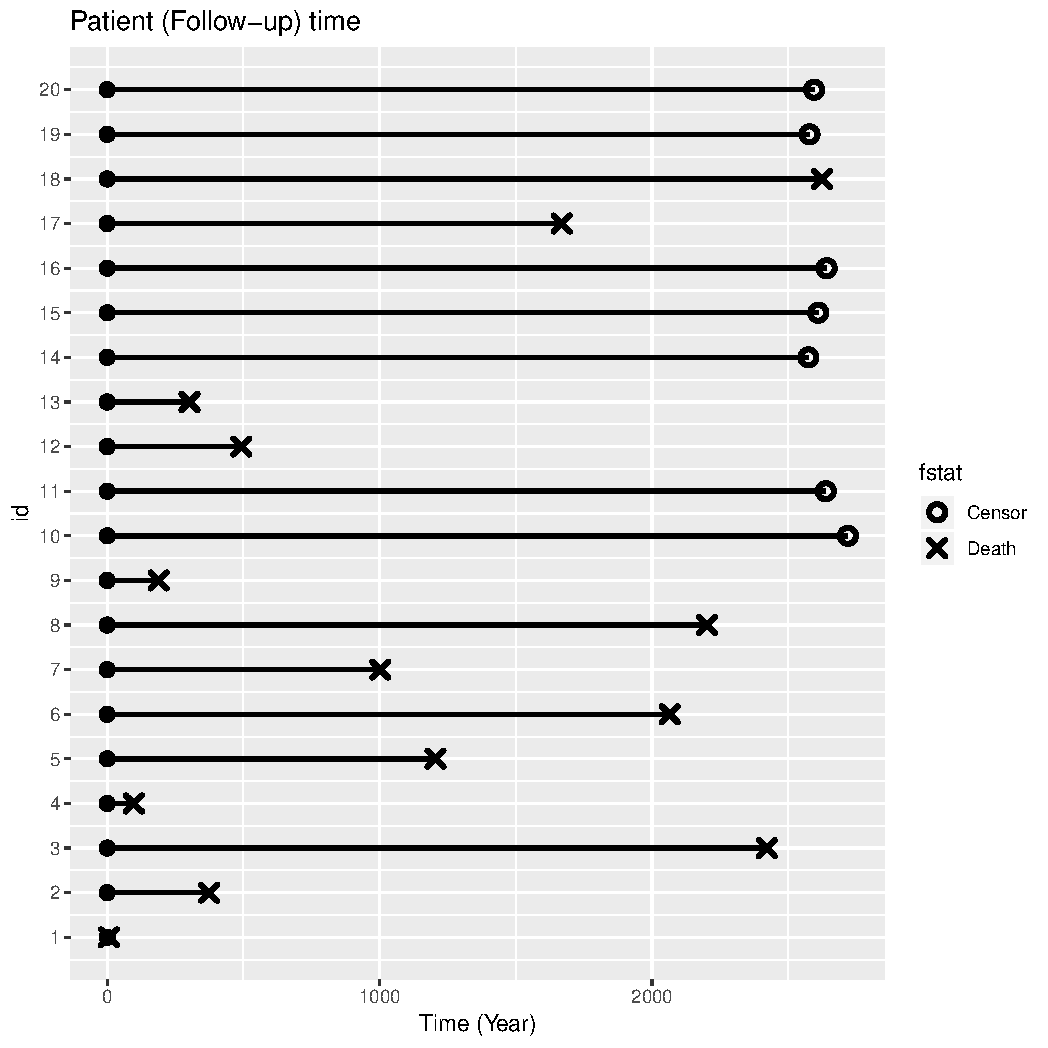
\includegraphics[scale = .3]{tab1-1-2}
  \end{center}
\end{frame}

\begin{frame}[fragile]
  \frametitle{WHAS}
  \begin{itemize}
  \item Patients are \emph{not} all recruited at exactly the same time.
  \item The end of study appear to be Jan. 05, 2003. 
\begin{knitrout}\scriptsize
\definecolor{shadecolor}{rgb}{0.969, 0.969, 0.969}\color{fgcolor}\begin{kframe}
\begin{alltt}
\hlstd{> }\hlkwd{max}\hlstd{(}\hlkwd{strptime}\hlstd{(whas100}\hlopt{$}\hlstd{foldate,} \hlkwc{format} \hlstd{=} \hlstr{"%m/%d/%Y"}\hlstd{))}
\end{alltt}
\begin{verbatim}
[1] "2003-01-05 CST"
\end{verbatim}
\end{kframe}
\end{knitrout}
  \item Patients remain alive at the end of study, 
    \begin{itemize}
    \item patient \# 10, 11, 14, 15, 16, etc.
    \end{itemize}
  \item or left the study by then are considered (right) censored.
    \begin{itemize}
    \item none in this study.
    \end{itemize}
  \item In the above figures, the \textbf{X} marks the events.
  \item There are two types of censoring:
    \begin{itemize}
    \item Informative; dropout related to the outcome
    \item Non-informative (indepndent); dropout not related to the outcome
    \end{itemize}
  \end{itemize}
\end{frame}

\begin{frame}[fragile]
  \frametitle{\texttt{Surv} objects}
  \begin{itemize}
  \item In this course, we will use $t$ to denote the duration (right figure).
  \item The \texttt{Surv} function in the \pkg{survival} package produces a special structure for survival data:
\begin{knitrout}\scriptsize
\definecolor{shadecolor}{rgb}{0.969, 0.969, 0.969}\color{fgcolor}\begin{kframe}
\begin{alltt}
\hlstd{> }\hlkwd{library}\hlstd{(survival)}
\hlstd{> }\hlkwd{args}\hlstd{(Surv)}
\end{alltt}
\begin{verbatim}
function (time, time2, event, type = c("right", "left", "interval", 
    "counting", "interval2", "mstate"), origin = 0) 
NULL
\end{verbatim}
\end{kframe}
\end{knitrout}
  \item Similar structure is adopted to several packages. 
    For examples,
\begin{knitrout}\scriptsize
\definecolor{shadecolor}{rgb}{0.969, 0.969, 0.969}\color{fgcolor}\begin{kframe}
\begin{alltt}
\hlstd{> }\hlkwd{args}\hlstd{(reda}\hlopt{::}\hlstd{Survr)}
\end{alltt}
\begin{verbatim}
function (ID, time, event, origin = 0, check = TRUE, ...) 
NULL
\end{verbatim}
\begin{alltt}
\hlstd{> }\hlkwd{args}\hlstd{(reReg}\hlopt{::}\hlstd{reSurv)}
\end{alltt}
\begin{verbatim}
function (time1, time2, id, event, status, origin = 0) 
NULL
\end{verbatim}
\end{kframe}
\end{knitrout}
  \end{itemize}
\end{frame}


\begin{frame}[fragile]
  \frametitle{\texttt{Surv} objects}
  \begin{itemize}
  \item For the WHAS, the \texttt{Surv} object is
\begin{knitrout}\scriptsize
\definecolor{shadecolor}{rgb}{0.969, 0.969, 0.969}\color{fgcolor}\begin{kframe}
\begin{alltt}
\hlstd{> }\hlstd{whas100} \hlopt \hlkwd{with}\hlstd{(}\hlkwd{Surv}\hlstd{(lenfol, fstat))}
\end{alltt}
\begin{verbatim}
  [1]    6   374  2421    98  1205  2065  1002  2201   189  2719+ 2638+
 [12]  492   302  2574+ 2610+ 2641+ 1669  2624  2578+ 2595+  123  2613+
 [23]  774  2012  2573+ 1874  2631+ 1907   538   104     6  1401  2710 
 [34]  841   148  2137+ 2190+ 2173+  461  2114+ 2157+ 2054+ 2124+ 2137+
 [45] 2031  2003+ 2074+  274  1984+ 1993+ 1939+ 1172    89   128  1939+
 [56]   14  1011  1497  1929+ 2084+  107   451  2183+ 1876+  936   363 
 [67] 1048  1889+ 2072+ 1879+ 1870+ 1859+ 2052+ 1846+ 2061+ 1912+ 1836+
 [78]  114  1557  1278  1836+ 1916+ 1934+ 1923+   44  1922+  274  1860+
 [89] 1806  2145+  182  2013+ 2174+ 1624   187  1883+ 1577    62  1969+
[100] 1054 
\end{verbatim}
\end{kframe}
\end{knitrout}
\item There are 100 observation times, e.g., $t_1$, \ldots, $t_{100}$.
\item Censored events are accompanied with $+$.
\item With the definition $Y$ is the exact event time, $C$ is the censoring time, then
  $T = \min(Y, C)$ is the \emph{observed} event time. 
\end{itemize}
\end{frame}

\begin{frame}[fragile]
  \frametitle{\texttt{Surv} objects}
  \begin{itemize}
  \item The \texttt{Surv} can be plotted with \R's generic function \texttt{plot}:
\begin{knitrout}\scriptsize
\definecolor{shadecolor}{rgb}{0.969, 0.969, 0.969}\color{fgcolor}\begin{kframe}
\begin{alltt}
\hlstd{> }\hlstd{whas100} \hlopt \hlkwd{with}\hlstd{(}\hlkwd{Surv}\hlstd{(lenfol, fstat))} \hlopt \hlstd{plot}
\end{alltt}
\end{kframe}
\end{knitrout}
    \begin{center}\vspace{-.1cm}
    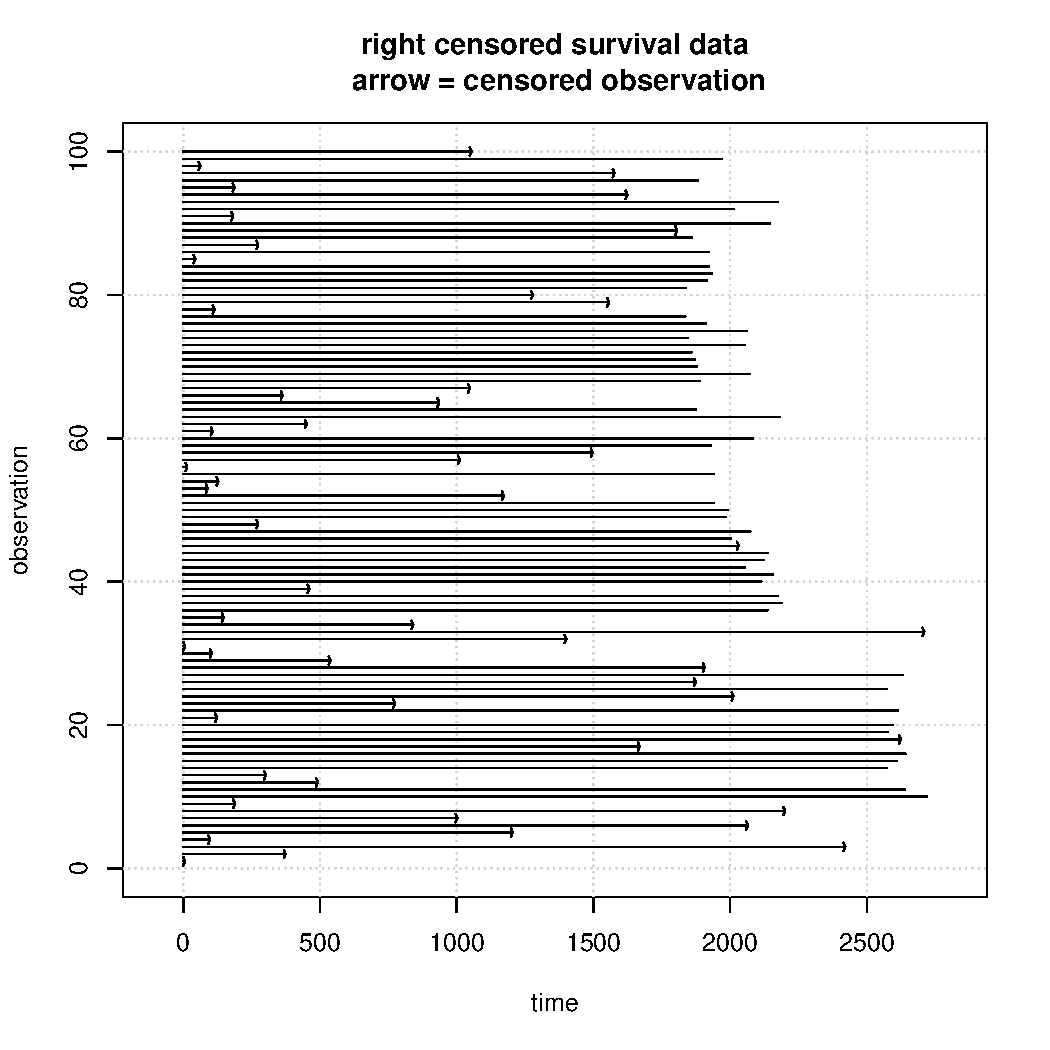
\includegraphics[scale = .43]{tab1-1-3}
    \end{center}
  \end{itemize}
\end{frame}

\begin{frame}[fragile]
  \frametitle{\texttt{Surv} objects}
  \begin{itemize}
  \item Another example of survival data that is subject to right censoring is the standard heart transplant program
\begin{knitrout}\scriptsize
\definecolor{shadecolor}{rgb}{0.969, 0.969, 0.969}\color{fgcolor}\begin{kframe}
\begin{alltt}
\hlstd{> }\hlkwd{data}\hlstd{(heart)}
\hlstd{> }\hlkwd{head}\hlstd{(heart)}
\end{alltt}
\begin{verbatim}
  start stop event        age      year surgery transplant id
1     0   50     1 -17.155373 0.1232033       0          0  1
2     0    6     1   3.835729 0.2546201       0          0  2
3     0    1     0   6.297057 0.2655715       0          0  3
4     1   16     1   6.297057 0.2655715       0          1  3
5     0   36     0  -7.737166 0.4900753       0          0  4
6    36   39     1  -7.737166 0.4900753       0          1  4
\end{verbatim}
\begin{alltt}
\hlstd{> }\hlstd{heart} \hlopt \hlkwd{with}\hlstd{(}\hlkwd{Surv}\hlstd{(start, stop, event))} \hlopt \hlkwd{head}\hlstd{(}\hlnum{14}\hlstd{)}
\end{alltt}
\begin{verbatim}
 [1] ( 0, 50]  ( 0,  6]  ( 0,  1+] ( 1, 16]  ( 0, 36+] (36, 39]  ( 0, 18] 
 [8] ( 0,  3]  ( 0, 51+] (51,675]  ( 0, 40]  ( 0, 85]  ( 0, 12+] (12, 58] 
\end{verbatim}
\end{kframe}
\end{knitrout}
  \item In this dataset, \code{start} is the entry time, \code{stop} is the exit time, 
    and \code{event} is the censoring indicator where death is indicated by \code{event = 1}.
  \item In this example, \code{Surv} displays the ``calendar time''.
  \end{itemize}
\end{frame}


\begin{frame}
  \frametitle{Other censoring}
  \begin{itemize}
  \item \empr{Left censoring} is encountered when the event of interest has already occurred when observation begins.
    \begin{itemize}
    \item Less common. 
    \item If the event of interest has already occurred when observation begins, 
      the subject is usually not selected in the study. 
      If these subjects are left out, this is referred to \emph{length biased sampling} or a special type of \emph{left truncation}.
    \end{itemize}
  \item \empr{Interval censoring} is when individuals are known to have experienced an event within an interval of time.
    \begin{itemize}
    \item When either end of the interval is undefined ($\infty$ or 0), 
      this reduced to either the left censoring or right censoring.
    \item When the length of interval is small (e.g., $\to0$), one might treats events as uncensored.
    \end{itemize}    
  \end{itemize}
\end{frame}  

\end{document}



  \item 
  \item After recruitment, patients are followed until they die, 
    or until a censoring event happens.
  \item 

    
  \begin{columns}
    \column{0.5\textwidth}
    \begin{center}
      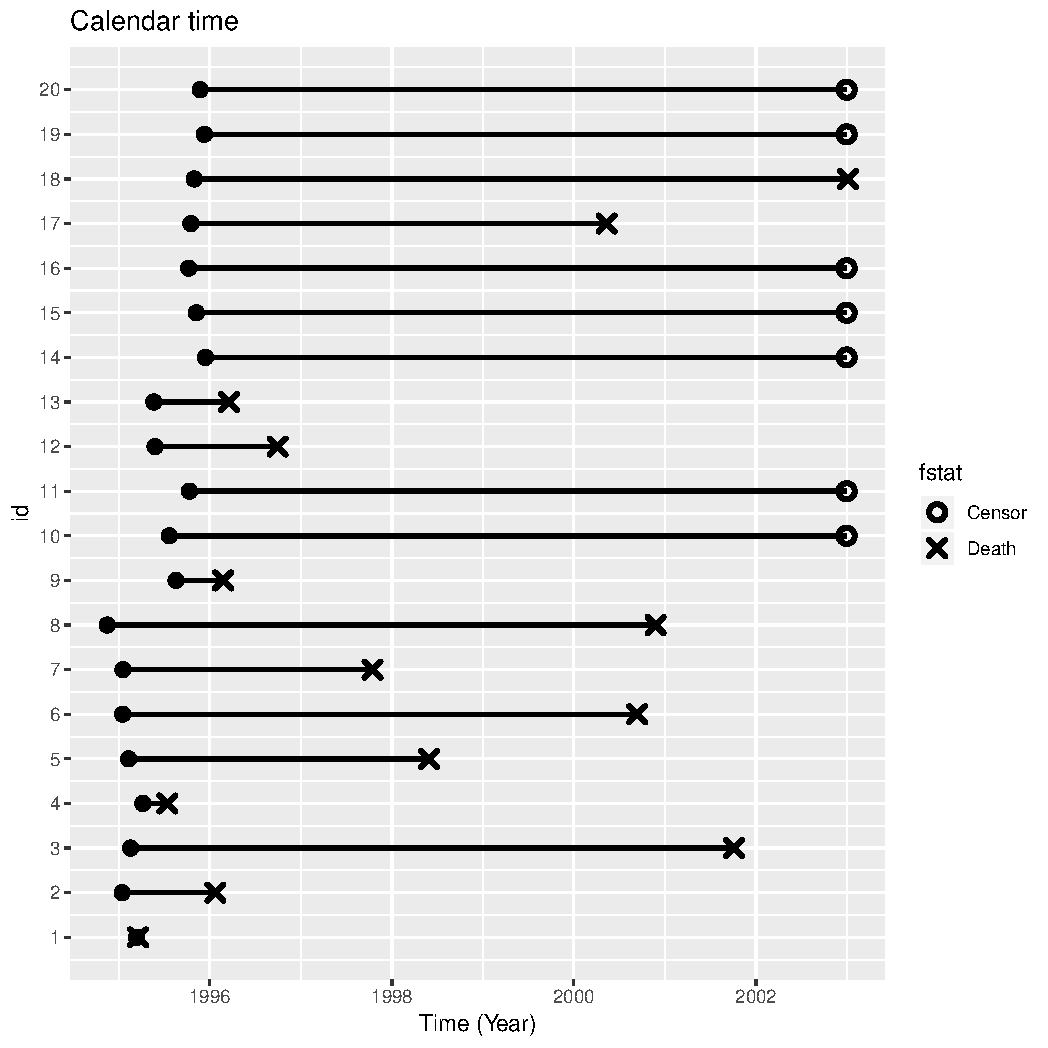
\includegraphics[scale = .35]{tab1-1-1}
    \end{center}
    \column{0.5\textwidth}
    \begin{itemize}
    \item The end of study is Jan. 05, 2003. 
    \item Patients remain alive at the end of study, or left the study by then are considered (right) censored.
    \end{itemize}
  \end{columns}
